\documentclass{ltjsarticle}
\usepackage{luatexja}
%Packages -----------------------
\usepackage{tikz}
\usepackage{listings}
\usepackage[euler]{textgreek}
\usepackage{enumitem}
\usepackage[margin=30mm]{geometry}
\usepackage{comment}
\usepackage{hyperref}
\usepackage{float}
\usepackage{textcomp}
\usepackage{xparse}
%Circuit ------------------------
\usepackage{amsmath,amssymb}
\usepackage{graphicx}
\usepackage{siunitx}
\usepackage{tikz}
\usepackage[siunitx, RPvoltages]{circuitikz}
%Circuit ------------------------
%Command ---–--------------------
\renewcommand{\figurename}{図}
\renewcommand{\baselinestretch}{1.1}
\renewcommand\lstlistingname{ソースコード}
\renewcommand\lstlistlistingname{ソースコード}
\lstset{
    numbers=left,
    basicstyle={\ttfamily},
    identifierstyle={\small},
    commentstyle={\smallitshape},
    keywordstyle={\small\bfseries},
    ndkeywordstyle={\small},
    stringstyle={\small\ttfamily},
    frame={tb},
    breaklines=true,
    columns=[l]{fullflexible},
    xrightmargin=0\zw,
    xleftmargin=3\zw,
    numberstyle={\scriptsize},
    stepnumber=1,
    %numbersep=1,
    lineskip=-0.5ex,
    keywordstyle=\color[HTML]{e10021},
    commentstyle=\color{gray},
    emph=CascadeObjectDetector,
    emphstyle=\color{blue}
}
%Command ------------------------
%Title   ------------------------
\title{実験レポートA3}
\author{東京大学工学部電気電子工学科 03210517\ 藤田 誠之 }
\date{May 6, 2021}
%Title   ------------------------

\begin{document}

\maketitle

\section{方法}
Xilinx Vivadoを用いてHDLシミュレーションを実行した.
\section{考察課題}
\subsection{1日目}
\subsubsection{AND回路の設計}

入力は2つのwire, 出力は1つのwireである. 2つの入力の論理積を出力する。
\begin{lstlisting}[caption=AND回路デザイン,language=verilog]
`timescale 1ns / 1ps
module and_gate (
    input wire inA,
    input wire inB,
    output wire out
);
    assign out = inA & inB;
endmodule
\end{lstlisting}
2入力の全部で4通りがある。テストベンチで100nsごとに入力を変化させた。
\begin{lstlisting}[caption=AND回路テストベンチ,language=verilog]
    module testbench;
    // parameter
    parameter CYCLE = 1000; // clock cycle
    parameter HALF_CYCLE = 500; // half cycle
    parameter DLY = 500; // delay
    // wire/reg
    reg clk;
    reg inA, inB;
    wire out_and_gate;
    // DUT module
    and_gate and_gate_0 (
        .inA(inA),
        .inB(inB),
        .out(out_and_gate)
    );
    // clock generator
    always begin
        clk = 1'b1;
        #(HALF_CYCLE) clk = 1'b0;
        #(HALF_CYCLE);
    end
    // test scenario
    initial begin
        // initialize
        inA = 1'b0; inB = 1'b0; 
        // for and_gate
        inA = 1'b0; inB = 1'b0;
        #100 $display("inA=%b inB=%b out=%b", inA, inB, out_and_gate);
        inA = 1'b1; inB = 1'b0;
        #100 $display("inA=%b inB=%b out=%b", inA, inB, out_and_gate);  
        inA = 1'b0; inB = 1'b1;
        #100 $display("inA=%b inB=%b out=%b", inA, inB, out_and_gate);  
        inA = 1'b1; inB = 1'b1;
        #100 $display("inA=%b inB=%b out=%b", inA, inB, out_and_gate);

        repeat(10) @(posedge clk); // repeat 10 times
        $finish;
    end
endmodule
\end{lstlisting}

\begin{figure}[H]
    \begin{center}
        \includegraphics[width=14cm]{figures/and.png}
        \caption{AND回路の波形}
    \end{center}
\end{figure}
inA, inBの値が(0,0),(1,0),(0,1),(1,1)と変化するにつれ出力が変化していることがわかる。outの値が1となっているのはinAとinBが1のときのみであり、論理積が表現できていることがわかる。

\subsubsection{NAND回路の設計}
入力は2つのwire, 出力は1つのwireである. 2つの入力をA,Bとすると、$\overline{A\dot B}$を出力する。

\begin{lstlisting}[caption=NANDデザイン,language=verilog]
`timescale 1ns / 1ps
module nand_gate (
    input wire inA,
    input wire inB,
    output wire out
);
    assign out = ~(inA & inB);
endmodule
\end{lstlisting}
テストベンチはAND回路のときと同じものを用いた。

\begin{figure}[H]
    \begin{center}
        \includegraphics[width=14cm]{figures/nand.png}
        \caption{NAND回路の波形}
    \end{center}
\end{figure}
inA, inBの値を(0,0),(1,0),(0,1),(1,1)と変化するにつれ出力が変化していることがわかる。outの値は(0,0),(1,0),(0,1)のときに1、(1,1)のときに0となっているが、これは$\overline{A\dot B}$をこの回路が正しく表現できていることがわかる。

\subsubsection{XOR回路の設計}
入力は2つのwire, 出力は1つのwireである。2つの入力をA,Bとすると、$A \oplus B$を出力する。
\begin{lstlisting}[caption=XORデザイン, language=verilog]
`timescale 1ns / 1ps
module xor_gate (
    input wire inA,
    input wire inB,
    output wire out
);
    assign out = inA ^ inB;
endmodule
\end{lstlisting}
テストベンチはAND回路のときと同じものを用いた。
\begin{figure}[H]
    \begin{center}
        \includegraphics[width=14cm]{figures/xor.png}
        \caption{XOR回路の波形}
    \end{center}
\end{figure}
inA, inBの値を(0,0),(1,0),(0,1),(1,1)と変化するにつれ出力が変化していることがわかる。outの値はinA,inBが(1,0),(0,1)のときに1となっており、$A \oplus B$が表現できていることがわかる。
\subsubsection{フリップフロップ回路の設計}
\tikzset{sr-ff/.style={flipflop, flipflop def={
    t1=D,t3 = {\texttt{CLK}}, t6=Q, c3=1, td=rst}},
}
以下のフリップフロップ回路は、出力を反転して入力に戻す。
\begin{figure}[H]
    \begin{center}
        \begin{circuitikz}[american currents]
            \ctikzset{american inductors}
            \draw (0,0)
            node[sr-ff](FF){} (FF.up)
            (FF.pin 1) -- ++(-0.5, 0)
            to[short] ++(0, 2)
            to[short] ++(1,0) node[not port, anchor = out, rotate = 180](not1){}
            (FF.pin 6) -- ++(0.5, 0)
            to[short] ++(0, 2)
            to (not1.in) -- ++(0.5,0);
        \end{circuitikz}
        \caption{FF回路}
    \end{center}
\end{figure}
このFF回路を作成する。入力はclkとrstの2つのwireであり、出力はoutのreg一つである。clkの立ち上がりで出力値がそれまでの出力値の反転となる。ただし、clkの立ち上がり時にrstが1であればoutの値は0のままとなる。また、rstの立ち上がり時にも出力値が0となる。なお、regを用いてoutの値を保持しておくことで、Dの入力のwireが不要となる。
\begin{lstlisting}[caption=インバータ付きFF回路デザイン,language=verilog]
`timescale 1ns / 1ps
module flipflop (
    input wire clk,
    input wire rst,
    output reg q
);
initial begin
    q = 1;
end
always @(posedge clk or posedge rst)
    if (rst) begin
        q <= 1'b0;
    end else begin
        q <= ~q;
    end
endmodule
\end{lstlisting}
clkは500msごとに値が1と0で切り替わる。適当なタイミングでrstの値を1とし、rstが想定通りに機能していることを確認する。
\begin{lstlisting}[caption=インバータ付きFF回路テストベンチ,language=verilog]
    module testbench_flipflop_not;
    // parameter
    parameter CYCLE = 1000; // clock cycle
    parameter HALF_CYCLE = 500; // half cycle
    parameter DLY = 500; // delay
    // wire/reg
    reg clk;
    reg rst;
    wire out;
    // DUT module
    flipflop_not flipflop_not0(
        .clk(clk),
        .rst(rst),
        .q(out)
    );
    // clock generator
    always begin
        clk = 1'b1;
        #(HALF_CYCLE) clk = 1'b0;
        #(HALF_CYCLE);
    end
    // test scenario
    initial begin   
        rst = 1'b0;
        #2200 $display("rst=%b out=%b", rst, out);
        rst = 1'b1;
        #400 $display("rst=%b out=%b", rst, out);  
        rst = 1'b0;
        #600 $display("rst=%b out=%b", rst, out);
        rst = 1'b1;
        #400 $display("rst=%b out=%b", rst, out);
        rst = 1'b0;
        #1200 $display("rst=%b out=%b", rst, out);
        rst = 1'b1;
        #400 $display("rst=%b out=%b", rst, out);
        rst = 1'b0;
        #1200 $display("rst=%b out=%b", rst, out);
        repeat(10) @(posedge clk); // repeat 10 times
        $finish;
    end
endmodule
\end{lstlisting}
\begin{figure}[H]
    \begin{center}
        \includegraphics[width=14cm]{figures/flipflop_not.png}
        \caption{インバータ付きフリップフロップ回路の波形}
    \end{center}
\end{figure}
波形を観察すると、設計通り、clkの立ち上がりでoutの値が反転しており、またrstの立ち上がりでoutの値が0となっていることがわかる。


\subsubsection{ラッチ回路の設計}
\tikzset{sr-ff2/.style={flipflop, flipflop def={
    t1=D,t3 = {\texttt{CLK}}, t6=Q, c3=1}},
}
以下のようなラッチ回路を作成する。
\begin{figure}[H]
    \begin{center}
        \begin{circuitikz}[american currents]
            \ctikzset{american inductors}
            \draw (0,0)
            node[sr-ff2](FF){Latch} (FF.up);
        \end{circuitikz}
        \caption{ラッチ回路}
    \end{center}
\end{figure}
入力はclkとDのwireの2つ、出力は1つのregである。クロックが1であれば出力の値がDの値となり、クロックが0になってもその直前の出力値を保持する。
\begin{lstlisting}[caption=ラッチ回路デザイン,language=verilog]
`timescale 1ns / 1ps
module latch (
    input wire clk,
    input wire D,
    output reg Q
);
    always @* begin
        if (clk==1'b1)
        Q = D;
    end
endmodule
\end{lstlisting}
clkは250msごとに切り替わる。Dを適当なタイミングで切り替え、out値の挙動を観察する。
\begin{lstlisting}[caption=*****,language=verilog]
module testbench_flipflop_not;
    // parameter
    parameter CYCLE = 1000; // clock cycle
    parameter HALF_CYCLE = 500; // half cycle
    parameter DLY = 500; // delay
    // wire/reg
    reg clk;
    reg rst;
    wire out;
    // DUT module
    flipflop_not flipflop_not0(
        .clk(clk),
        .rst(rst),
        .q(out)
    );
    // clock generator
    always begin
        clk = 1'b1;
        #(HALF_CYCLE) clk = 1'b0;
        #(HALF_CYCLE);
    end
    // test scenario
    initial begin
        rst = 1'b0;
        #2200 $display("rst=%b out=%b", rst, out);
        rst = 1'b1;
        #400 $display("rst=%b out=%b", rst, out);  
        rst = 1'b0;
        #600 $display("rst=%b out=%b", rst, out);
        rst = 1'b1;
        #400 $display("rst=%b out=%b", rst, out);
        rst = 1'b0;
        #1200 $display("rst=%b out=%b", rst, out);
        rst = 1'b1;
        #400 $display("rst=%b out=%b", rst, out);
        rst = 1'b0;
        #1200 $display("rst=%b out=%b", rst, out);
        repeat(10) @(posedge clk); // repeat 10 times
        $finish;
    end
endmodule
\end{lstlisting}
\begin{figure}[H]
    \begin{center}
        \includegraphics[width=15cm]{figures/flipflop_latch.png}
        \caption{ラッチ回路の波形}
    \end{center}
\end{figure}
図ではinAとなっているものが入力Dである。設計通り、clkの立ち上がりのときのAの値が出力として保持されていることがわかる。

\subsection{2日目}
\subsubsection{ハーフアダーの設計}
ハーフアダーは1bitの加算を桁上げまで含めて行う。
\begin{figure}[H]
    \begin{center}
        \begin{circuitikz}[american currents]
            \tikzset{halfadder/.style={draw, thick, minimum height=1.5cm, minimum width=2cm, rounded corners = 0.3cm}}
            \node[halfadder] (A) at (0,0) {};
            \draw ($(A.north west)!.5!(A.west)$) to[short,l_=A,-o] ++(-1,0)
            ($(A.south west)!.5!(A.west)$) to[short,l_=B,-o] ++(-1,0)
            ($(A.north east)!.5!(A.east)$) to[short,l=S,-o] ++(1,0)
            ($(A.south east)!.5!(A.east)$) to[short,l=C,-o] ++(1,0);
        \end{circuitikz}
        \caption{ハーフアダー}
    \end{center}
\end{figure}
入力は2つのwireであり、出力は2つのwireである。入力をA,Bとすると$S=A\oplus B$、$C=A\dot B$を出力する。前日に作成したAND回路やXOR回路も使用している。
\begin{lstlisting}[caption=ハーフアダーデザイン,language=verilog]
`timescale 1ns / 1ps
module HalfAdder(
    input wire A,
    input wire B,
    output wire S,
    output wire C
    );
    xor_gate U0 (.inA(A), .inB(B), .out(S));
    and_gate U1 (.inA(A), .inB(B), .out(C));    
endmodule
\end{lstlisting}
4通りの2入力を入力し、出力を見る。
\begin{lstlisting}[caption=ハーフアダーテストベンチ,language=verilog]
    module HalfAddertestbench;
    // parameter
    parameter CYCLE = 1000; // clock cycle
    parameter HALF_CYCLE = 500; // half cycle
    parameter DLY = 500; // delay
    // wire/reg
    reg clk;
    reg  A,B;
    wire C,S;
    // DUT module
    HalfAdder  HalfAdder0(
        .A(A),
        .B(B),
        .C(C),
        .S(S)
    );    
    // clock generator
    always begin
        clk = 1'b1;
        #(HALF_CYCLE) clk = 1'b0;
        #(HALF_CYCLE);
    end
    // test scenario
    initial begin
        // for and_gate
        A = 1'b0; B = 1'b0;
        #100 $display("A=%b B=%b C=%b S=%b", A, B, C, S);
        A = 1'b1; B = 1'b0;
        #100 $display("A=%b B=%b C=%b S=%b", A, B, C, S); 
        A = 1'b0; B = 1'b1;
        #100 $display("A=%b B=%b C=%b S=%b", A, B, C, S);  
        A = 1'b1; B = 1'b1;
        #100 $display("A=%b B=%b C=%b S=%b", A, B, C, S);
        repeat(10) @(posedge clk); // repeat 10 times
        $finish;
    end
endmodule
\end{lstlisting}
\begin{figure}[H]
    \begin{center}
        \includegraphics[width=8cm]{figures/halfadder.png}
        \caption{ハーフアダー回路の波形}
    \end{center}
\end{figure}
図から値の名前が消えてしまっているが、上から順にclk、A, B, C, Sである。実際に、$C=A\oplus B$、$S=A\dot B$を表現することができていることがわかる。
\subsubsection{フルアダーの設計}
フルアダーは、ハーフアダーに過去の繰り上げの情報を付加して計算する。
\begin{figure}[H]
    \begin{center}
        \begin{circuitikz}[american currents]
            \tikzset{fulladder/.style={draw, thick, minimum height=1.5cm, minimum width=2cm, rounded corners = 0.3cm}}
            \node[fulladder] (A) at (0,0) {};
            \draw ($(A.north west)!.5!(A.west)$) to[short,l_=A,-o] ++(-1,0)
            ($(A.west)!.5!(A.west)$) to[short,l_=B,-o] ++(-1,0)
            ($(A.south west)!.5!(A.west)$) to[short,l_=$C_{in}$,-o] ++(-1,0)
            ($(A.north east)!.5!(A.east)$) to[short,l=S,-o] ++(1,0)
            ($(A.south east)!.5!(A.east)$) to[short,l=$C_{out}$,-o] ++(1,0);
        \end{circuitikz}
        \caption{ハーフアダー}
    \end{center}
\end{figure}
入力は$A$、$B$、$C_{in}$の3つのwireであり、出力は$S$、$C_{in}$の2つのwireである。ハーフアダーを以下の様に2つつなげることにより、完結に表現することができる。
\begin{figure}[H]
    \begin{center}
        \begin{circuitikz}[american currents]
            \tikzset{fulladder/.style={draw, thick, minimum height=1.5cm, minimum width=2cm, rounded corners = 0.3cm}}
            \node[fulladder] (A) at (0,0) {};
            \node[fulladder] (B) at (4,0) {};
            \draw ($(A.north west)!.5!(A.west)$) to[short,l_=A,-o] ++(-1,0)
            ($(A.south west)!.5!(A.west)$) to[short,l_=B,-o] ++(-1,0)
            ($(A.north east)!.5!(A.east)$) to[short] ++(1,0)
            to ($(B.north west)!.5!(B.west)$) -- ++ (0,0)
            ($(B.north east)!.5!(B.east)$) to[short] ++(3,0)
            to[short, l=S, -o] ++(1,0)
            ($(A.south east)!.5!(A.east)$) to[short] ++(0.5,0)
            to[short] ++(0,-1.57)
            to[short] ++(5,0) node[or port, anchor = in 2](or1){}
            ($(B.south west)!.5!(B.west)$) to[short] ++(-0.5,0)
            to[short] ++(0, -1)
            to[short] ++(-3.5,0)
            to[short,l_=$C_{in}$,-o] ++(-1,0)
            ($(B.south east)!.5!(B.east)$) to[short] ++(0.5,0)
            to[short] ++(0,-1)
            to (or1.in 1) -- ++(0,0)
            (or1.out) to[short,l=$C_{out}$,-o] ++(1,0);
        \end{circuitikz}
        \caption{ハーフアダー}
    \end{center}
\end{figure}
\begin{lstlisting}[caption=フルアダーデザイン,language=verilog]
`timescale 1ns / 1ps
module Fulladder(
    input wire CI,
    input wire A,
    input wire B,
    output wire S,
    output wire CO
    );
    wire w1;
    wire w2;
    wire w3;
    HalfAdder HalfAdder0(
        .A(A),
        .B(B),
        .S(w1),
        .C(w2)
        );
    HalfAdder HalfAdder1(
        .A(w1),
        .B(CI),
        .S(S),
        .C(w3)
        );
    assign CO = w2|w3;
endmodule
\end{lstlisting}
$A$,$B$,$C_{in}$に関してそれぞれ0,1の8通りを表現する。
\begin{lstlisting}[caption=フルアダーテストベンチ,language=verilog]
module FullAddertestbench;
    // parameter
    parameter CYCLE = 1000; // clock cycle
    parameter HALF_CYCLE = 500; // half cycle
    parameter DLY = 500; // delay
    // wire/reg
    reg clk;
    reg  A,B,CI;
    wire CO,S;
    // DUT module
    Fulladder  Fulladder0(
        .A(A),
        .B(B),
        .CI(CI),
        .CO(CO),
        .S(S)
    );    
    // clock generator
    always begin
        clk = 1'b1;
        #(HALF_CYCLE) clk = 1'b0;
        #(HALF_CYCLE);
    end
    // test scenario
    initial begin
        // for and_gate
        A = 1'b0; B = 1'b0; CI = 1'b0;
        #100 $display("A=%b B=%b CI=%b CO=%b S=%b ", A, B, CI, CO, S);
        A = 1'b1; B = 1'b0; CI = 1'b0;
        #100 $display("A=%b B=%b CI=%b CO=%b S=%b", A, B, CI, CO, S); 
        A = 1'b0; B = 1'b1; CI = 1'b0;
        #100 $display("A=%b B=%b CI=%b CO=%b S=%b", A, B, CI, CO, S);  
        A = 1'b1; B = 1'b1; CI = 1'b0;
        #100 $display("A=%b B=%b CI=%b CO=%b S=%b", A, B, CI, CO, S);
        A = 1'b0; B = 1'b0; CI = 1'b1;
        #100 $display("A=%b B=%b CI=%b CO=%b S=%b ", A, B, CI, CO, S);
        A = 1'b1; B = 1'b0; CI = 1'b1;
        #100 $display("A=%b B=%b CI=%b CO=%b S=%b", A, B, CI, CO, S); 
        A = 1'b0; B = 1'b1; CI = 1'b1;
        #100 $display("A=%b B=%b CI=%b CO=%b S=%b", A, B, CI, CO, S);  
        A = 1'b1; B = 1'b1; CI = 1'b1;
        #100 $display("A=%b B=%b CI=%b CO=%b S=%b", A, B, CI, CO, S);
        repeat(10) @(posedge clk); // repeat 10 times
        $finish;
    end
endmodule
\end{lstlisting}
\begin{figure}[H]
    \begin{center}
        \includegraphics[width=10cm]{figures/fulladder.png}
        \caption{フルアダー回路の波形}
    \end{center}
\end{figure}
上から$A$、$B$、$C_{in}$、$S$、$C_{out}$である。入力に合致した値が得られていることがわかる。
\subsubsection{4-bit リップルキャリアアダーの設計}
フルアダーを4つ並べて繋げたものである。

\begin{figure}[H]
    \begin{center}
        \begin{circuitikz}[american currents]
            \tikzset{one bit adder/.style={muxdemux, muxdemux def={Lh=4, NL=2, Rh=2, NR=1, NB=1, NT=1, w=1.5, inset w=0.5, inset Lh=2, inset Rh=0, square pins=1}}}
            \draw
            node[one bit adder, rotate=-90](D) at (0,0) {A}
            node[one bit adder, rotate=-90](C) at (3,0) {B}
            node[one bit adder, rotate=-90](B) at (6,0) {C}
            node[one bit adder, rotate=-90](A) at (9,0) {D}
            (A.tpin 1) to(B.bpin 1) -- ++(0,0)
            (B.tpin 1) to(C.bpin 1) -- ++(0,0)
            (C.tpin 1) to(D.bpin 1) -- ++(0,0);
        \end{circuitikz}
        \caption{4-bit リップルキャリアアダー}
    \end{center}
\end{figure}
Aの初期値は0とし、4bitの16進数として表示された値をそれぞれの桁の値をそれぞれ対応するフルアダーに入力する。Dの$C_{out}$は最終的な計算結果のキャリーとなることがわかる。
\begin{lstlisting}[caption=4-bit リップルキャリアアダーデザイン,language=verilog]
`timescale 1ns / 1ps
module Addripple4(
    input wire [3:0]a,
    input wire [3:0]b,
    output wire [3:0]s,
    output wire of
    );
    Fulladder Fulladder0(.S(s[0]),.B(b[0]),.A(a[0]),.CI(0),.CO(w0));
    Fulladder Fulladder1(.S(s[1]),.B(b[1]),.A(a[1]),.CI(w0),.CO(w1));
    Fulladder Fulladder2(.S(s[2]),.B(b[2]),.A(a[2]),.CI(w1),.CO(w2));
    Fulladder Fulladder3(.S(s[3]),.B(b[3]),.A(a[3]),.CI(w2),.CO(of));
endmodule
\end{lstlisting}
AとBが4bitずつの$2^8$通りを計算するテストベンチを作成した。
\begin{lstlisting}[caption=*****,language=verilog]
    module testbench_addripple4;
    // parameter
    parameter CYCLE = 1000; // clock cycle
    parameter HALF_CYCLE = 500; // half cycle
    parameter DLY = 500; // delay
    // wire/reg
    reg clk;
    reg  [3:0]A,B;
    wire C;
    wire [3:0]S;
    // DUT module
    Addripple4 Addripple4_0(A,B,S,C);
    // clock generator
    always begin
        clk = 1'b1;
        #(HALF_CYCLE) clk = 1'b0;
        #(HALF_CYCLE);
    end
     integer i;
     integer j;
    // test scenario
    initial begin
        // initialize
        A = 4'b0; B = 4'b0;
        // for add4_gate
        for(i = 0; i<16; i = i+1) begin
          for(j = 0; j<16; j = j+1)begin
            A = i; B = j;
            #40 $display("A=%b B=%b C=%b S=%b", A, B, C, S);
          end        
        end
        repeat(10) @(posedge clk); // repeat 10 times
        $finish;
    end
endmodule
\end{lstlisting}
\begin{figure}[H]
    \begin{center}
        \includegraphics[width=14cm]{figures/addripple4.png}
        \caption{4-bit リップルキャリアアダー}
    \end{center}
\end{figure}
256通りすべてを網羅した。入力と出力A,B,Sは16進法で表されており、また計算全体としてキャリーが発生する場合はCがと1となっており、これがオーバーフローの検出として機能していることがわかる。
\subsubsection{4-bit アダーの設計}
フルアダーの組み合わせとしてではなく、1つの回路として4-bitの加算器を作成する。
\begin{lstlisting}[caption=4-bit アダー,language=verilog]
`timescale 1ns / 1ps
module Add4(a,b,s,carry); 
    input [3:0]a,b;
    output [3:0]s;
    output carry;
    assign {carry, s} = a + b;
endmodule    
\end{lstlisting}
4-bitリップルキャリアアダーに比べ、とても簡潔に表現できている。テストベンチは4-bit リップルキャリアアダーと同じものを用いた。
\begin{figure}[H]
    \begin{center}
        \includegraphics[width=14cm]{figures/addripple4.png}
        \caption{フルアダー回路の波形}
    \end{center}
\end{figure}
結果、同じテストベンチ4-bitリップルキャリアアダーと同一の結果が得られた。
\subsection{3日目}
\subsubsection{動作の違いの調査}
以下の回路は入力が2つのwire、出力が2つのwireの回路である。
\begin{lstlisting}[caption=*****,language=verilog]
`timescale 1ns / 1ps
module example (
    input wire inA,
    input wire clk,
    output wire out1,
    output wire out2
);
    reg out1_reg, out2_reg;
    always @(posedge clk) begin
        out1_reg <= inA;
    end
    always @(*) begin
        out2_reg <= inA;
    end
    assign out1 = out1_reg;
    assign out2 = out2_reg;
endmodule
\end{lstlisting}
ソースコードを調べると、posedge内でout1regを決めていることがわかるため、フリップフロップはout1であると予想できる。これを確かめるテストベンチを作成した。40msごとに入力を切り替えている。
\begin{lstlisting}[caption=*****,language=verilog]
module testbench_example;
  wire	o1,o2;
  reg clk;
  reg	a;
  always begin
        clk = 1'b1;
        #50 clk = 1'b0;
        #50;
  end
  integer i = 0;
  initial begin
	a <= 0;
	for (i = 0; i < 40; i = i+1) begin
	   a <= i%2;
	   #28;
	end
	repeat(2) @(posedge clk);
	$finish;
  end
  example example0( a,clk,o1,o2 );
endmodule
\end{lstlisting}
\begin{figure}[H]
    \begin{center}
        \includegraphics[width=15cm]{figures/example.png}
        \caption{example回路の波形}
    \end{center}
\end{figure}
実際、out1がフリップフロップ回路であることが確認できた。
\subsubsection{基本的な順序回路の設計}
以下のような挙動を示す回路を設計する。つまり、出力の初期値は0であり、clkが立ち上がりの瞬間にSTARTが1であれば1を1クロック分出力、その後3クロックごとに1クロック分だけ出力を1とするというものである。また、clk立ち上げ時にstartが1であればそれまでの挙動に考えなくその時点で出力を1とし、また3クロックごとに出力を1とする。
\begin{figure}[H]
    \begin{center}
        \includegraphics[width=10cm]{figures/junjo.png}
        \caption{順序回路}
    \end{center}
\end{figure}
状態遷移図は以下のようになる。
\begin{center}
    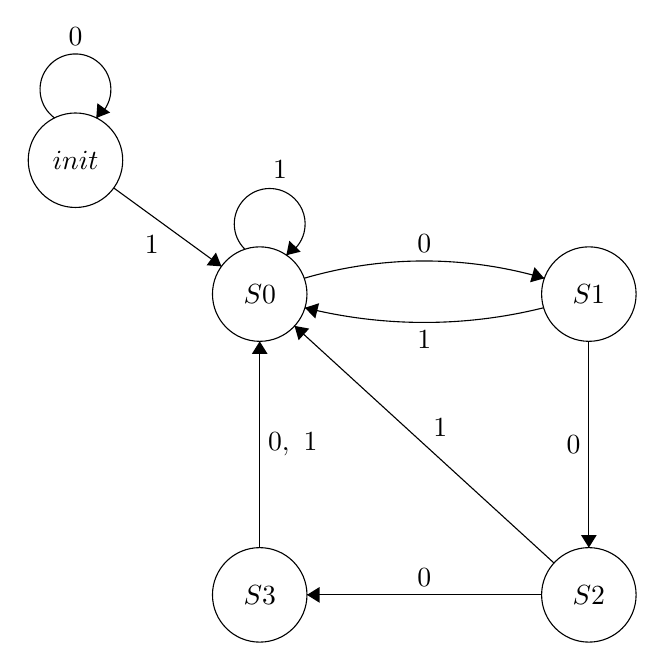
\begin{tikzpicture}[scale=0.2]
    \tikzstyle{every node}+=[inner sep=0pt]
    \draw [black] (17.5,-13.6) circle (3);
    \draw (17.5,-13.6) node {$init$};
    \draw [black] (29.2,-22.1) circle (3);
    \draw (29.2,-22.1) node {$S0$};
    \draw [black] (50.1,-22.1) circle (3);
    \draw (50.1,-22.1) node {$S1$};
    \draw [black] (50.1,-41.2) circle (3);
    \draw (50.1,-41.2) node {$S2$};
    \draw [black] (29.2,-41.2) circle (3);
    \draw (29.2,-41.2) node {$S3$};
    \draw [black] (32.025,-21.095) arc (106.40005:73.59995:27.006);
    \fill [black] (47.27,-21.1) -- (46.65,-20.39) -- (46.37,-21.35);
    \draw (39.65,-19.5) node [above] {$0$};
    \draw [black] (50.1,-25.1) -- (50.1,-38.2);
    \fill [black] (50.1,-38.2) -- (50.6,-37.4) -- (49.6,-37.4);
    \draw (49.6,-31.65) node [left] {$0$};
    \draw [black] (47.1,-41.2) -- (32.2,-41.2);
    \fill [black] (32.2,-41.2) -- (33,-41.7) -- (33,-40.7);
    \draw (39.65,-40.7) node [above] {$0$};
    \draw [black] (29.2,-38.2) -- (29.2,-25.1);
    \fill [black] (29.2,-25.1) -- (28.7,-25.9) -- (29.7,-25.9);
    \draw (29.7,-31.65) node [right] {$0,\mbox{ }1$};
    \draw [black] (47.229,-22.967) arc (-75.95396:-104.04604:31.228);
    \fill [black] (32.07,-22.97) -- (32.73,-23.65) -- (32.97,-22.68);
    \draw (39.65,-24.4) node [below] {$1$};
    \draw [black] (47.89,-39.18) -- (31.41,-24.12);
    \fill [black] (31.41,-24.12) -- (31.67,-25.03) -- (32.34,-24.29);
    \draw (40.66,-31.16) node [above] {$1$};
    \draw [black] (28.268,-19.261) arc (225.90428:-62.09572:2.25);
    \draw (30.49,-14.82) node [above] {$1$};
    \fill [black] (30.89,-19.63) -- (31.8,-19.41) -- (31.08,-18.71);
    \draw [black] (16.177,-10.92) arc (234:-54:2.25);
    \draw (17.5,-6.35) node [above] {$0$};
    \fill [black] (18.82,-10.92) -- (19.7,-10.57) -- (18.89,-9.98);
    \draw [black] (19.93,-15.36) -- (26.77,-20.34);
    \fill [black] (26.77,-20.34) -- (26.42,-19.46) -- (25.83,-20.27);
    \draw (22.35,-18.35) node [below] {$1$};
    \end{tikzpicture}
\end{center}
clk立ち上がり時のSTARTの値によって状態が遷移し、状態がS0のときのみ1を出力する。\\
入力がclkとstartの2つのwire、出力が1つの回路を作成した。posedgeによりclkの立ち上がりを検知、iによりクロックの立ち上がり回数を記録し、iが3になったら1を出力すると同時にiを0とする。また、clk立ち上がり時にSTARTが1のときは1を出力すると同時にiを0とする。また、最初のSTARTの信号までは0を出力するため、これまでのSTARTの有無を記録している。
\begin{lstlisting}[caption=順序回路デザイン,language=verilog]
`timescale 1ns / 1ps
module sequence(
        input wire start,
        input wire clk,
        output wire out
    );
    reg [1:0]i;
    reg out_reg;
    reg start_reg;
    initial begin
        i <= 0;
        start_reg <= 0;
        out_reg <= 0;
    end
    always @(posedge clk) begin
        if (start == 1 || start_reg == 1) begin
            start_reg <= 1;
            if (start == 1 || i == 3) begin 
                out_reg <= 1;
                i <= 0;
            end else begin
                out_reg <= 0;
                i <= i+1;
            end
        end
    end
    assign out = out_reg;
endmodule
\end{lstlisting}
テストベンチを作成し、START信号が送られると3クロックごとに出力が0となっていることが確認できれば良い。32ns毎に1/7の確率でランダムにclkが1となるようにし、波形を観測した。
\begin{lstlisting}[caption=順序回路テストベンチ,language=verilog]
`timescale 1ns / 1ps
module test_sequence_rst;
  wire	out;
  reg rst;
  reg clk;
  reg	in;
  always begin
        clk = 1'b1;
        #50 clk = 1'b0;
        #50;
  end
  integer i = 0;
  initial begin
	in <= 0;
	rst <= 0;
	#50 in<=1;
	#100 in<=0;
	for (i = 0; i < 200; i = i+1) begin
	   if ($random%4 == 0) begin
	       rst <= 1;
	   end else rst <= 0;
	   #10;
	   rst <= 0;
	   #90;
	end
	repeat(2) @(posedge clk);
	$finish;
  end
  sequence_rst sequence_rst0( in,clk,rst,out );
endmodule
\end{lstlisting}
上で述べた設計通りに動作していることが確認できた。
\subsubsection{非同期リセット機能の追加}
上記の回路では、クロックの立ち上がり時にSTART信号が1となっていないと出力がリセットされない。つまり、START信号が1になったとしても、次のclkの立ち上がりまでに0に戻っていれば検知されない。そこで、STARTのwireとは別に、そのような信号を送ってもリセットができるようなRST信号を加えた回路が以下である。
\begin{lstlisting}[caption=rst機能付き順序回路デザイン,language=verilog]
`timescale 1ns / 1ps
module test_sequence_rst;
  wire	out_sync;
  wire out_async;
  reg start;
  reg rst;
  reg clk;
  reg in;
  always begin
        clk = 1'b1;
        #50 clk = 1'b0;
        #50;
  end
  integer i = 0;
  initial begin
	in <= 0;
	rst <= 0;
	start <= 0;
	#50 in<=1;start<=1;rst<=1;
	#95 in<=0;start<=0;rst<=0;
	for (i = 0; i < 200; i = i+1) begin
	   if ($random%8 == 0) begin
	       rst = 1; start = 1;
	   end else begin rst = 0; start=0; end
	   #10;
	   rst = 0; start = 0;
	   #40;
	end
	repeat(2) @(posedge clk);
	$finish;
  end
  sequence_rst sequence_rst0( in,clk,rst,out_async );
  sequence sequence0(start,clk,out_sync);
endmodule
\end{lstlisting}
2節のテストベンチに加え、rst信号を適当なタイミングで送るようなテストベンチを組み、挙動を確認する。
\begin{lstlisting}[caption=リセット付き順序回路デザイン,language=verilog]
'timescale 1ns / 1ps
module sequence_rst(
        input wire start,
        input wire clk,
        input wire rst,
        output wire out
    );
    reg [1:0]i;
    reg out_reg;
    reg rst_reg;
    reg start_reg;
    initial begin
        i <= 0;
        start_reg <= 0;
        rst_reg <= 0;
        out_reg <= 0;
    end
    always @(posedge clk) begin
        if(start == 1 || start_reg == 1 || (rst_reg == 1 && start_reg == 1)) begin
            start_reg <= 1;
            if(start == 1 || rst_reg == 1 || i == 3) begin
                out_reg <= 1;
                i <= 0;
                rst_reg <= 0;
            end else begin
                out_reg <= 0;
                i <= i+1;
            end
        end
    end
    always @(posedge rst) begin
        rst_reg <= 1;
    end
    assign out = out_reg;
endmodule
\end{lstlisting}
\begin{lstlisting}[caption=リセット付き順序回路テストベンチ,language=verilog]
'timescale 1ns / 1psmodule test_sequence_rst2;
module test_sequence_rst2;
    wire out_sync;
    wire out_async;
    reg start;
    reg rst;
    reg clk;
    reg in;
    always begin
        clk = 1'b1;
        #50 clk = 1'b0;
        #50;
    end
    integer i = 0;
    initial begin
        in <= 0;
        rst <= 0;
        start <= 0;
        #50 in <= 1; start <= 1; rst <= 1;
        #95 in = 0; start <= 0; rst <= 0;
        for(i = 0; i < 200; i = i + 1) begin
            if($random%7 == 0) begin
                rst = 1; start = 1;
            end else begin rst = 0; start = 0; end
            #10;
            rst = 0; start = 0;
            #40;
        end
        repeat(2) @(posedge clk);
        $finish;
    end
    sequence_rst sequence_rst0(in,clk,rst,out_async);
    sequence sequence0(start,clk,out_sync);
endmodule
\end{lstlisting}
設計通りに、STARTはclkが立ち上がるときに1であればリセット、RSTは一瞬でも1となればリセットされるというように、設計通りに回路が動いていることがわかる。
\subsection{4日目}
\subsubsection{メモリ読み出し回路の設計とシミュレーション}
クロックを用い、クロックの立ち上がりごとにmem.hexファイルに保存された16進法の1桁の数字を読み出す。アドレスは0から始め、clkの立ち上がりごとに1増やしている。なお、次の節の課題において用いる機能を考え、メモリ読み出し時に次の数字を取得するか、次の次の数字を取得するかを選択できるようにしている。
\begin{lstlisting}[caption=メモリ読み出し回路デザイン,language=verilog]
`timescale 1ns / 1ps
module read_4 ( 
    input wire clk,
    output wire [3:0] out_data
);
    reg [3:0] mem [0:31];
    reg [3:0] mem_out;
    reg [4:0] addr_reg;
    initial begin
        $readmemh("C:/Users/tromb/OneDrive/Desktop/files/Day4/mem.hex", mem);
        addr_reg = 0;
    end
    always @(posedge clk) begin
        mem_out <= mem[addr_reg];
        addr_reg = addr_reg + 1;
          // synchronous read
    end
    assign out_data = mem_out;  
endmodule
\end{lstlisting}
\begin{lstlisting}[caption=メモリ読み出し回路テストベンチ,language=verilog]
`timescale 1ns / 1ps
module testbench;
	reg clk;
	wire [3:0] out;
	always begin
		clk = 1'b1;
		#50 clk = 1'b0;
		#50;
	end
	read_4 read_a_digit(clk,out);
	always @(posedge clk) begin
	   if (out !== 4'bx)
	      $display("%x", out);
end
endmodule
\end{lstlisting}
実際に、mem.hexに保存されている数字が1クロックごとに読み出されていることがわかる。
\subsubsection{メモリ比較回路の設計とシミュレーション}
上記の読み出し回路を編集し、1クロックごとに次の数字と次の次の数字を読み出し、上で作成した4-bitリップルキャリアアダーを用いて2つの数字の和とキャリーの有無を計算する。オーバーフローがある場合はoutofが1となる。また、似たコードを用いてref.hexを1クロックごとに同時に読み出し、計算結果と一致するかどうかを調べ出力する。また、間違いが会った場合は標準出力にそのアドレスが表示される。
\begin{lstlisting}[caption=メモリ比較回路デザイン,language=verilog]
`timescale 1ns / 1ps
module read_ref ( 
    input wire clk,
    output wire [3:0] out_data,
    output wire [4:0] out_addr
);
    reg [3:0] mem [0:31];
    reg [3:0] mem_out;
    reg [4:0] addr_reg;
    initial begin
        $readmemh("C:/Users/tromb/OneDrive/Desktop/files/Day4/ref.hex", mem);
        addr_reg = 0;
    end
    always @(posedge clk) begin
        mem_out <= mem[addr_reg];
        addr_reg = addr_reg + 1;
          // synchronous read
    end
    assign out_data = mem_out;
    assign out_addr = addr_reg;
endmodule
\end{lstlisting}
\begin{lstlisting}[caption=メモリ比較回路テストベンチ,language=verilog]
`timescale 1ns / 1ps
module testbench;
	reg clk;
	wire [3:0] out;
	wire out_of;
	wire [3:0] out_ref;
	wire [4:0] out_addr;
	always begin
		clk = 1'b1;
		#50 clk = 1'b0;
		#50;
	end
	initial begin  
	end
	add2digits add21(clk,out,out_of);
	read_ref readit(clk,out_ref,out_addr);
	always @(posedge clk) begin
	   if (out !== 4'bx)
	   	  if (out !== out_ref)
	        $display("%x", out_addr);
end
endmodule
\end{lstlisting}
計算結果と、読みだした結果と、それらの一致不一致が表現されていることがわかる。
\section{参考文献}
『title』\url{<url>} 2021年n月m日アクセス
\end{document}